\subsubsection{UC0: Scenario principale} \label{sec:UC0}
\begin{description}
\item[\em{descrizione }]L'utente ha avviato il sistema il quale è pronto a rispondere agli eventi. L'utente può scegliere di accedere alla calibrazione delle telecamere, accedere alla loro configurazione, oppure generare le statistiche a partire dai dati di tracking attualmente presenti nel sistema (figura ~\ref{fig:uc0})
\item[\em{flusso principale degli eventi }] \mbox{}
\begin{enumerate}
\item L'utente può calibrare le telecamere (\hyperref[sec:uc1]{UC1}) 
\item L'utente può configurare le telecamere (\hyperref[sec:uc2]{UC2})
\item L'utente può generare e visualizzare le statistiche (\hyperref[sec:uc3]{UC3})
\end{enumerate}
\item[\em{precondizione }] Il sistema è avviato e funzionante
\end{description}

\begin{figure}[htpb] 
\centering 
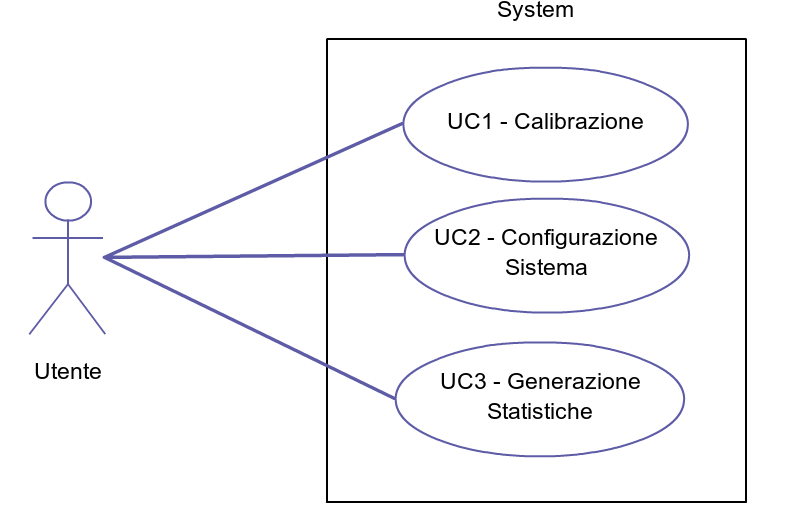
\includegraphics[scale=0.4]{./images/uc0.png} 
\caption{UC0 - Scenario principale} 
\label{fig:uc0}
\end{figure} 

\subsubsection{UC1: Calibrazione telecamere} \label{sec:UC1}
\begin{description}
\item[\em{descrizione }]L'utente può iniziare la calibrazione delle telecamere, oppure può visualizzare un video \textit{undistorted} che usa i parametri di calibrazione per correggere i frame prodotti dal video. (figura ~\ref{fig:uc1})
\item[\em{flusso principale degli eventi }] \mbox{}
\begin{enumerate}
\item L'utente può iniziare la calibrazione (\hyperref[sec:uc1.1]{UC1.1}) 
\item L'utente può visualizzare il video corretto con i parametri di calibrazione (\hyperref[sec:uc1.2]{UC1.2})
\end{enumerate}
\item[\em{precondizione }] Il sistema è avviato e funzionante
\end{description}

\begin{figure}[htpb] 
\centering 
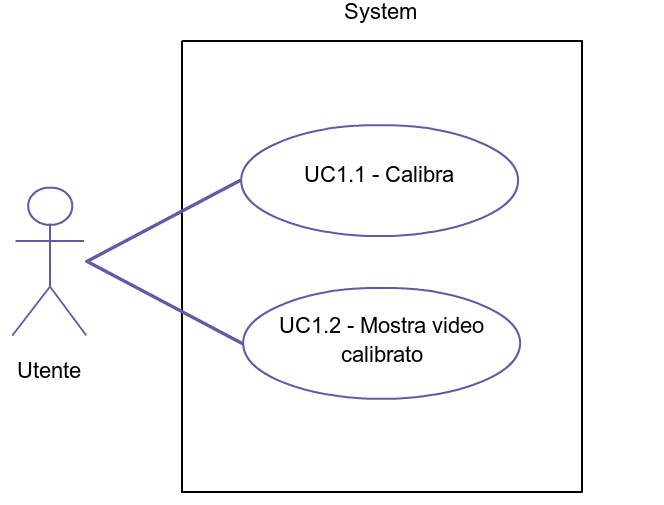
\includegraphics[scale=0.4]{./images/uc1.png} 
\caption{UC1 - Calibrazione telecamere} 
\label{fig:uc1}
\end{figure} 

\subsubsection{UC1.1: Calibra} \label{sec:UC1.1}
\begin{description}
\item[\em{descrizione }]L'utente sta selezionando le opzioni per la calibrazione delle telecamere. Può selezionare: numero di span spot della scacchiera, numero di frame da scartare durante la calibrazione, indirizzo IP nella rete della camera da calibrare, e poi iniziare l'effettiva calibrazione. (figura ~\ref{fig:uc1.1})
\item[\em{flusso principale degli eventi }] \mbox{}
\begin{enumerate}
\item L'utente seleziona il numero di span spot (\hyperref[sec:uc1.1.1]{UC1.1.1})
\item L'utente seleziona il numero frame da scartare (\hyperref[sec:uc1.1.2]{UC1.1.2})
\item L'utente seleziona l'indirizzo della camera da calibrare (\hyperref[sec:uc1.1.3]{UC1.1.3})
\item L'utente avvia la calibrazione calibrare (\hyperref[sec:uc1.1.4]{UC1.1.4})
\end{enumerate}
\item[\em{postcondizione }] I file che contengono i file di calibrazione della telecamera (extrinsics e instrinsics) sono stati generati e salvati nel file system
\item[\em{scenari alternativi }] \mbox{} 
\begin{enumerate} 
\item L'utente interrompe la procedura, il sistema torna in attesa di eventi
\item La procedura di calibrazione fallisce, il sistema segnala l'errore e torna in attesa di eventi
\end{enumerate}
\end{description}

\begin{figure}[htpb] 
\centering 
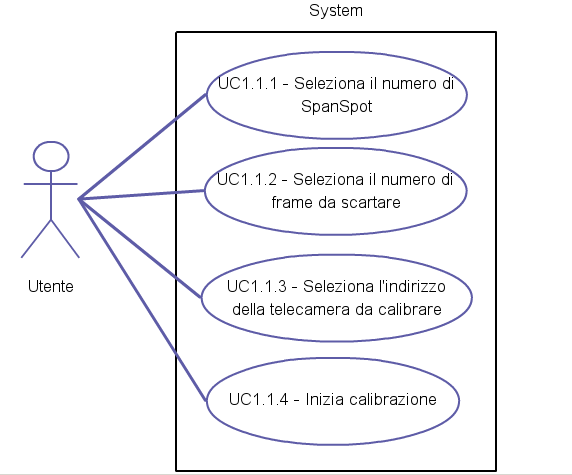
\includegraphics[scale=0.4]{./images/uc11.png} 
\caption{UC1.1 - Calibra} 
\label{fig:uc1.1}
\end{figure} 

\subsubsection{UC1.1.1: Seleziona il numero di span spot} \label{sec:UC1.1.1}
\begin{description}
\item[\em{descrizione }]L'utente seleziona il numero di span spot per la calibrazione
\item[\em{postcondizione }] Il sistema conosce il numero di span spot da utilizzare nella calibrazione
\item[\em{scenari alternativi }] \mbox{} 
\begin{enumerate} 
\item L'utente interrompe la procedura, il sistema ritorna in attesa di eventi
\end{enumerate}
\end{description}

\subsubsection{UC1.1.2: Seleziona il numero di frame da scartare} \label{sec:UC1.1.2}
\begin{description}
\item[\em{descrizione }]L'utente seleziona il numero di frame da scartare per la calibrazione
\item[\em{precondizione }] L'utente ha già selezionato il numero di span spot
\item[\em{postcondizione }] Il sistema conosce il numero di frame da scartare nella calibrazione
\item[\em{scenari alternativi }] \mbox{} 
\begin{enumerate} 
\item L'utente interrompe la procedura, il sistema ritorna in attesa di eventi
\end{enumerate}
\end{description}

\subsubsection{UC1.1.3: Inserisce l'indirizzo della telecamera da calibrare} \label{sec:UC1.1.3}
\begin{description}
\item[\em{descrizione }]L'utente inserisce l'indirizzo della telecamera da calibrare
\item[\em{precondizione }] L'utente ha già selezionato il numero di span spot e il numero di frame da scartare nella calibrazione
\item[\em{postcondizione }] Il sistema conosce l'indirizzo della telecamera da calibrare
\item[\em{scenari alternativi }] \mbox{} 
\begin{enumerate} 
\item L'utente interrompe la procedura, il sistema ritorna in attesa di eventi
\end{enumerate}
\end{description}

\subsubsection{UC1.1.4: Inizia calibrazione} \label{sec:UC1.1.4}
\begin{description}
\item[\em{descrizione }]L'utente inizia la calibrazione effettiva
\item[\em{precondizione }] L'utente ha già selezionato le opzioni di calibrazione (UC1.1.1 - UC1.1.2 - UC1.1.3), il sistema quindi conosce i parametri da utilizzare
\item[\em{postcondizione }] Il sistema genera i file di calibrazione intrinsics ed extrinsics e li salva nel file system
\item[\em{scenari alternativi }] \mbox{} 
\begin{enumerate} 
\item La calibrazione non termina con successo quindi l'operazione viene interrotta e l'errore segnalato. Il sistema ritorna in attesa di eventi
\end{enumerate}
\end{description}

\subsubsection{UC1.2: Mostra video calibrato} \label{sec:UC1.2}
\begin{description}
\item[\em{descrizione }]L'utente visualizza il video corretto con i valori di calibrazione
\item[\em{precondizione }] L'utente ha già effettuato con successo la generazione dei file di calibrazione che sono presenti nel sistema
\end{description}

\subsubsection{UC2: Configurazione telecamere} \label{sec:UC2}
\begin{description}
\item[\em{descrizione }]L'utente può impostare le opzioni di configurazione delle telecamere, aggiungendone di nuove, rimuovendole, modificandole. Può inoltre ottenere i file necessari alla configurazione, convertendo un file .DXF in .PNG, salvando un frame dalla telecamera, o calcolare la \textit{homography matrix} (figura ~\ref{fig:uc2})
\item[\em{flusso principale degli eventi }] \mbox{}
\begin{enumerate}
\item L'utente inserisce una nuova telecamera nel sistema (\hyperref[sec:uc2.1]{UC2.1})
\item L'utente rimuove una telecamera esistente (\hyperref[sec:uc2.2]{UC2.2})
\item L'utente modifica la configurazione di una telecamera (\hyperref[sec:uc2.3]{UC2.3})
\item L'utente cattura e salva un frame della telecamera (\hyperref[sec:uc2.4]{UC2.4})
\item L'utente converte un file .DXF in .PNG (\hyperref[sec:uc2.5]{UC2.5})
\item L'utente calcola la matrice omografica relativa ad una telecamera (\hyperref[sec:uc2.6]{UC2.6})
\item L'utente seleziona una telecamera (\hyperref[sec:uc2.7]{UC2.7})
\end{enumerate}
\item[\em{precondizione }] Il sistema è avviato e funzionante.
\end{description}

\begin{figure}[htpb] 
\centering 
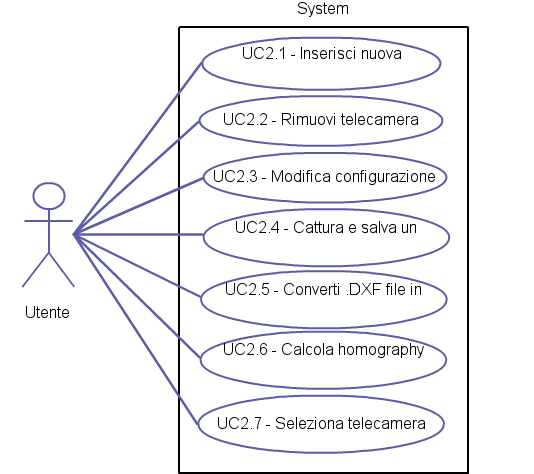
\includegraphics[scale=0.4]{./images/uc2.png} 
\caption{UC2 - Configurazione telecamere} 
\label{fig:uc2}
\end{figure} 

\subsubsection{UC2.1: Inserisci nuova} \label{sec:UC2.1}
\begin{description}
\item[\em{descrizione }]L'utente inserisce il nome della nuova telecamera
\item[\em{postcondizione }] Il sistema ha inserito la nuova telecamera nel database
\item[\em{scenari alternativi }] \mbox{} 
\begin{enumerate} 
\item Il nome inserito non è valido, il sistema interrompe l'operazione e torna in attesa di eventi.
\end{enumerate}
\end{description}

\subsubsection{UC2.2: Rimuovi telecamera} \label{sec:UC2.2}
\begin{description}
\item[\em{descrizione }]L'utente rimuove la telecamera selezionata
\item[\em{precondizione }] L'utente ha selezionato una telecamera tra quelle esistenti
\item[\em{postcondizione }] Il sistema ha rimosso la telecamera dal database
\end{description}

\subsubsection{UC2.3: Modifica configurazione} \label{sec:UC2.3}
\begin{description}
\item[\em{descrizione }]L'utente ha selezionato una telecamera e ne modifica le opzioni di configurazione, quali: file extrinsics, intrinsics, valore dell'altezza del frame, valore della larghezza del frame, percorso del file contentente la \textit{homography matrix} (figura ~\ref{fig:uc23}).
\item[\em{flusso principale degli eventi }] \mbox{}
\begin{enumerate}
\item L'utente modifica il percorso del file di calibrazione \textit{extrinsics} (\hyperref[sec:uc2.3.1]{UC2.3.1})
\item L'utente r modifica il percorso del file di calibrazione \textit{intrinsics} (\hyperref[sec:uc2.3.2]{UC2.3.2})
\item L'utente modifica il valore dell'altezza del frame (\hyperref[sec:uc2.3.3]{UC2.3.3})
\item L'utente modifica il valore della larghezza del frame (\hyperref[sec:uc2.3.4]{UC2.3.4})
\item L'utente modifica il percorso del file di configurazione contenente la \textit{homography matrix} (\hyperref[sec:uc2.3.5]{UC2.3.5})
\end{enumerate}
\item[\em{precondizione }] L'utente ha selezionato una telecamera tra quelle esistenti
\item[\em{scenari alternativi }] \mbox{} 
\begin{enumerate} 
\item L'utente interrompe la modifica, il sistema ritorna in attesa di eventi
\end{enumerate}
\end{description}

\begin{figure}[htpb] 
\centering 
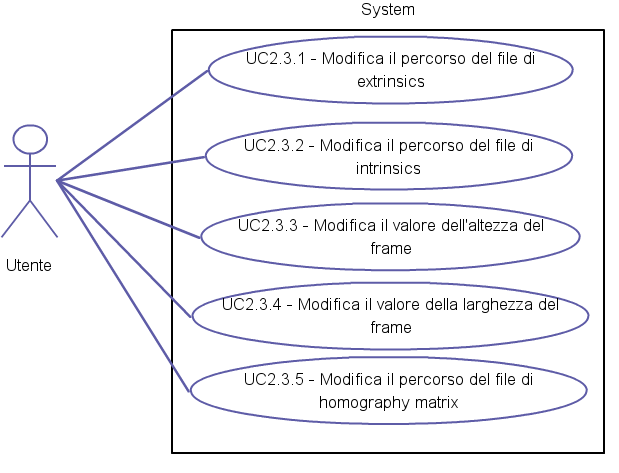
\includegraphics[scale=0.4]{./images/uc23.png} 
\caption{UC2.3 - Modifica configurazione} 
\label{fig:uc2.3}
\end{figure} 

\subsubsection{UC2.3.1: Modifica il percorso del file di extrinsics} \label{sec:UC2.3.1}
\begin{description}
\item[\em{descrizione }]L'utente seleziona un file nel file system che contiene i valori \textit{extrinsics} di calibrazione.
\item[\em{postcondizione }] Il sistema ha modificato il corrispondente valore della telecamera nel database
\item[\em{scenari alternativi }] \mbox{} 
\begin{enumerate} 
\item L'utente interrompe la selezione del file, il sistema ritorna in attesa di eventi
\end{enumerate}
\end{description}

\subsubsection{UC2.3.2: Modifica il percorso del file di intrinsics} \label{sec:UC2.3.2}
\begin{description}
\item[\em{descrizione }]L'utente seleziona un file nel file system che contiene i valori \textit{intrinsics} di calibrazione.
\item[\em{postcondizione }] Il sistema ha modificato il corrispondente valore della telecamera nel database
\item[\em{scenari alternativi }] \mbox{} 
\begin{enumerate} 
\item L'utente interrompe la selezione del file, il sistema ritorna in attesa di eventi
\end{enumerate}
\end{description}

\subsubsection{UC2.3.3: Modifica il valore dell'altezza del frame} \label{sec:UC2.3.3}
\begin{description}
\item[\em{descrizione }]L'utente seleziona un valore per l'altezza del frame della telecamera.
\item[\em{postcondizione }] Il sistema ha modificato il corrispondente valore della telecamera nel database
\end{description}

\subsubsection{UC2.3.4: Modifica il valore della larghezza del frame} \label{sec:UC2.3.4}
\begin{description}
\item[\em{descrizione }]L'utente seleziona un valore per la larghezza del frame della telecamera.
\item[\em{postcondizione }] Il sistema ha modificato il corrispondente valore della telecamera nel database
\end{description}

\subsubsection{UC2.3.5: Modifica il percorso del file di homography matrix} \label{sec:UC2.3.5}
\begin{description}
\item[\em{descrizione }]L'utente seleziona un file nel file system che contiene i valori che descrivono la \textit{homography matrix} utilizzata per la traduzione delle coordinate.
\item[\em{postcondizione }] Il sistema ha modificato il corrispondente valore della telecamera nel database
\item[\em{scenari alternativi }] \mbox{} 
\begin{enumerate} 
\item L'utente interrompe la selezione del file, il sistema ritorna in attesa di eventi
\end{enumerate}
\end{description}

\subsubsection{UC2.4: Cattura e salva un frame della telecamera} \label{sec:UC2.4}
\begin{description}
\item[\em{descrizione }]L'utente indica al sistema di attivare la telecamera selezionata, catturare un frame e salvarlo.
\item[\em{precondizione }] L'utente ha selezionato una telecamera tra quelle esistenti
\item[\em{postcondizione }] Il frame della telecamera selezionata è stato salvato nel file system
\item[\em{scenari alternativi }] \mbox{} 
\begin{enumerate} 
\item La telecamera non è raggiungibile, il sistema interrompe l'operazione segnala l'errore e ritorna in attesa di eventi
\end{enumerate}
\end{description}

\subsubsection{UC2.5: Converti .DXF file in .PNG} \label{sec:UC2.5}
\begin{description}
\item[\em{descrizione }]L'utente seleziona nel file system un file .DXF da convertire in formato .PNG 
\item[\em{postcondizione }] Il file selezionato è stato convertito in un immagine che riproduce il contenuto del .DXF
\end{description}

\subsubsection{UC2.6: Calcola homography matrix} \label{sec:UC2.6}
\begin{description}
\item[\em{descrizione }]L'utente calcola la homography matrix per una particolare telecamera configurata.
\item[\em{postcondizione }] Il file che contiene la \textit{homography matrix} è stato calcolato e salvato nel file system
\end{description}

\subsubsection{UC2.7: Seleziona telecamera} \label{sec:UC2.7}
\begin{description}
\item[\em{descrizione }]L'utente seleziona una telecamera tra la lista di telecamere presenti nel sistema
\item[\em{postcondizione }] La telecamera indicata diventa selezionata e quindi \textbf{attiva}
\end{description}

\subsubsection{UC3: Generazione statistiche} \label{sec:UC3}
\begin{description}
\item[\em{descrizione }]L'utente può visualizzare le statistiche relative ai dati presenti nel sistema. Può effettuare la conversione dei dati \textit{raw}, visualizzare l'\textit{heatmap}, o le statistiche (figura ~\ref{fig:uc3})
\item[\em{flusso principale degli eventi }] \mbox{}
\begin{enumerate}
\item L'utente seleziona la trasformazione dei dati di tracciamento presenti nel sistema (\hyperref[sec:uc3.1]{UC3.1})
\item L'utente seleziona la generazione dell'heatmap (\hyperref[sec:uc3.2]{UC3.2})
\item L'utente seleziona la generazione delle statistiche (\hyperref[sec:uc3.3]{UC3.3})
\end{enumerate}
\item[\em{precondizione }] Il sistema è avviato e funzionante.
\end{description}

\begin{figure}[htpb] 
\centering 
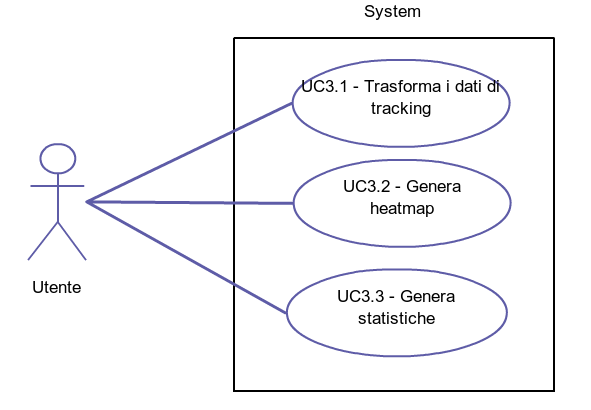
\includegraphics[scale=0.4]{./images/uc3.png} 
\caption{UC3 - Generazione statistiche} 
\label{fig:uc3}
\end{figure} 

\subsubsection{UC3.1: Trasforma i dati di tracking} \label{sec:UC3.1}
\begin{description}
\item[\em{descrizione }]L'utente indica al sistema di eseguire la trasformazione dei dati \textit{raw} di tracking
\item[\em{postcondizione }] Il sistema ha trasformato i dati presenti nel database ed ha salvato i dati trasformati.
\item[\em{scenari alternativi }] \mbox{} 
\begin{enumerate} 
\item La trasformazione fallisce, il sistema segnala l'errore e torna in attesa di eventi
\end{enumerate}
\end{description}

\subsubsection{UC3.2: Genera heatmap} \label{sec:UC3.2}
\begin{description}
\item[\em{descrizione }]L'utente indica al sistema di generare l'heatmap con la rappresentazione grafica dei dati di tracking
\item[\em{postcondizione }] Il sistema elabora i dati presenti nel database generando l'heatmap e salvandola nel file system.
\item[\em{scenari alternativi }] \mbox{} 
\begin{enumerate} 
\item La generazione fallisce, il sistema segnala l'errore e torna nello stato di attesa.
\end{enumerate}
\end{description}

\subsubsection{UC3.3: Genera statistiche} \label{sec:UC3.3}
\begin{description}
\item[\em{descrizione }]L'utente indica al sistema di generare le statistiche relative ai dati presenti
\item[\em{postcondizione }] Il sistema ha generato le statistiche e le ha salvate nel database
\item[\em{scenari alternativi }] \mbox{} 
\begin{enumerate} 
\item La generazione fallisce, il sistema segnala l'errore e torna nello stato di attesa.
\end{enumerate}
\end{description}
